\documentclass[1p]{elsarticle_modified}
%\bibliographystyle{elsarticle-num}

%\usepackage[colorlinks]{hyperref}
%\usepackage{abbrmath_seonhwa} %\Abb, \Ascr, \Acal ,\Abf, \Afrak
\usepackage{amsfonts}
\usepackage{amssymb}
\usepackage{amsmath}
\usepackage{amsthm}
\usepackage{scalefnt}
\usepackage{amsbsy}
\usepackage{kotex}
\usepackage{caption}
\usepackage{subfig}
\usepackage{color}
\usepackage{graphicx}
\usepackage{xcolor} %% white, black, red, green, blue, cyan, magenta, yellow
\usepackage{float}
\usepackage{setspace}
\usepackage{hyperref}

\usepackage{tikz}
\usetikzlibrary{arrows}

\usepackage{multirow}
\usepackage{array} % fixed length table
\usepackage{hhline}

%%%%%%%%%%%%%%%%%%%%%
\makeatletter
\renewcommand*\env@matrix[1][\arraystretch]{%
	\edef\arraystretch{#1}%
	\hskip -\arraycolsep
	\let\@ifnextchar\new@ifnextchar
	\array{*\c@MaxMatrixCols c}}
\makeatother %https://tex.stackexchange.com/questions/14071/how-can-i-increase-the-line-spacing-in-a-matrix
%%%%%%%%%%%%%%%

\usepackage[normalem]{ulem}

\newcommand{\msout}[1]{\ifmmode\text{\sout{\ensuremath{#1}}}\else\sout{#1}\fi}
%SOURCE: \msout is \stkout macro in https://tex.stackexchange.com/questions/20609/strikeout-in-math-mode

\newcommand{\cancel}[1]{
	\ifmmode
	{\color{red}\msout{#1}}
	\else
	{\color{red}\sout{#1}}
	\fi
}

\newcommand{\add}[1]{
	{\color{blue}\uwave{#1}}
}

\newcommand{\replace}[2]{
	\ifmmode
	{\color{red}\msout{#1}}{\color{blue}\uwave{#2}}
	\else
	{\color{red}\sout{#1}}{\color{blue}\uwave{#2}}
	\fi
}

\newcommand{\Sol}{\mathcal{S}} %segment
\newcommand{\D}{D} %diagram
\newcommand{\A}{\mathcal{A}} %arc


%%%%%%%%%%%%%%%%%%%%%%%%%%%%%5 test

\def\sl{\operatorname{\textup{SL}}(2,\Cbb)}
\def\psl{\operatorname{\textup{PSL}}(2,\Cbb)}
\def\quan{\mkern 1mu \triangleright \mkern 1mu}

\theoremstyle{definition}
\newtheorem{thm}{Theorem}[section]
\newtheorem{prop}[thm]{Proposition}
\newtheorem{lem}[thm]{Lemma}
\newtheorem{ques}[thm]{Question}
\newtheorem{cor}[thm]{Corollary}
\newtheorem{defn}[thm]{Definition}
\newtheorem{exam}[thm]{Example}
\newtheorem{rmk}[thm]{Remark}
\newtheorem{alg}[thm]{Algorithm}

\newcommand{\I}{\sqrt{-1}}
\begin{document}

%\begin{frontmatter}
%
%\title{Boundary parabolic representations of knots up to 8 crossings}
%
%%% Group authors per affiliation:
%\author{Yunhi Cho} 
%\address{Department of Mathematics, University of Seoul, Seoul, Korea}
%\ead{yhcho@uos.ac.kr}
%
%
%\author{Seonhwa Kim} %\fnref{s_kim}}
%\address{Center for Geometry and Physics, Institute for Basic Science, Pohang, 37673, Korea}
%\ead{ryeona17@ibs.re.kr}
%
%\author{Hyuk Kim}
%\address{Department of Mathematical Sciences, Seoul National University, Seoul 08826, Korea}
%\ead{hyukkim@snu.ac.kr}
%
%\author{Seokbeom Yoon}
%\address{Department of Mathematical Sciences, Seoul National University, Seoul, 08826,  Korea}
%\ead{sbyoon15@snu.ac.kr}
%
%\begin{abstract}
%We find all boundary parabolic representation of knots up to 8 crossings.
%
%\end{abstract}
%\begin{keyword}
%    \MSC[2010] 57M25 
%\end{keyword}
%
%\end{frontmatter}

%\linenumbers
%\tableofcontents
%
\newcommand\colored[1]{\textcolor{white}{\rule[-0.35ex]{0.8em}{1.4ex}}\kern-0.8em\color{red} #1}%
%\newcommand\colored[1]{\textcolor{white}{ #1}\kern-2.17ex	\textcolor{white}{ #1}\kern-1.81ex	\textcolor{white}{ #1}\kern-2.15ex\color{red}#1	}

{\Large $\underline{11a_{284}~(K11a_{284})}$}

\setlength{\tabcolsep}{10pt}
\renewcommand{\arraystretch}{1.6}
\vspace{1cm}\begin{tabular}{m{100pt}>{\centering\arraybackslash}m{274pt}}
\multirow{5}{120pt}{
	\centering
	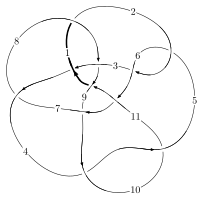
\includegraphics[width=112pt]{../../../GIT/diagram.site/Diagrams/png/533_11a_284.png}\\
\ \ \ A knot diagram\footnotemark}&
\allowdisplaybreaks
\textbf{Linearized knot diagam} \\
\cline{2-2}
 &
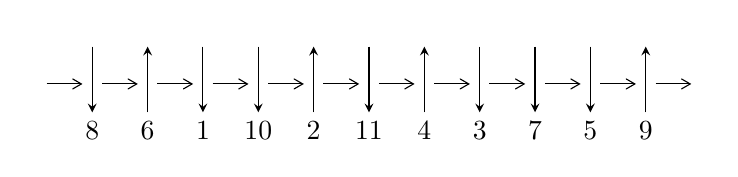
\begin{tikzpicture}[x=20pt, y=17pt]
	% nodes
	\node (C0) at (0, 0) {};
	\node (C1) at (1, 0) {};
	\node (C1U) at (1, +1) {};
	\node (C1D) at (1, -1) {8};

	\node (C2) at (2, 0) {};
	\node (C2U) at (2, +1) {};
	\node (C2D) at (2, -1) {6};

	\node (C3) at (3, 0) {};
	\node (C3U) at (3, +1) {};
	\node (C3D) at (3, -1) {1};

	\node (C4) at (4, 0) {};
	\node (C4U) at (4, +1) {};
	\node (C4D) at (4, -1) {10};

	\node (C5) at (5, 0) {};
	\node (C5U) at (5, +1) {};
	\node (C5D) at (5, -1) {2};

	\node (C6) at (6, 0) {};
	\node (C6U) at (6, +1) {};
	\node (C6D) at (6, -1) {11};

	\node (C7) at (7, 0) {};
	\node (C7U) at (7, +1) {};
	\node (C7D) at (7, -1) {4};

	\node (C8) at (8, 0) {};
	\node (C8U) at (8, +1) {};
	\node (C8D) at (8, -1) {3};

	\node (C9) at (9, 0) {};
	\node (C9U) at (9, +1) {};
	\node (C9D) at (9, -1) {7};

	\node (C10) at (10, 0) {};
	\node (C10U) at (10, +1) {};
	\node (C10D) at (10, -1) {5};

	\node (C11) at (11, 0) {};
	\node (C11U) at (11, +1) {};
	\node (C11D) at (11, -1) {9};
	\node (C12) at (12, 0) {};

	% arrows
	\draw[->,>={angle 60}]
	(C0) edge (C1) (C1) edge (C2) (C2) edge (C3) (C3) edge (C4) (C4) edge (C5) (C5) edge (C6) (C6) edge (C7) (C7) edge (C8) (C8) edge (C9) (C9) edge (C10) (C10) edge (C11) (C11) edge (C12) ;	\draw[->,>=stealth]
	(C1U) edge (C1D) (C2D) edge (C2U) (C3U) edge (C3D) (C4U) edge (C4D) (C5D) edge (C5U) (C6U) edge (C6D) (C7D) edge (C7U) (C8U) edge (C8D) (C9U) edge (C9D) (C10U) edge (C10D) (C11D) edge (C11U) ;
	\end{tikzpicture} \\
\hhline{~~} \\& 
\textbf{Solving Sequence} \\ \cline{2-2} 
 &
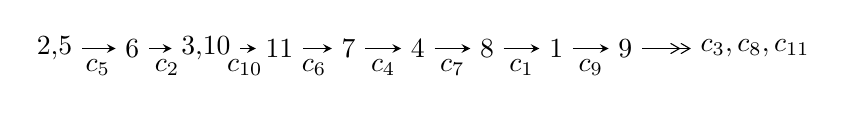
\begin{tikzpicture}[x=25pt, y=7pt]
	% node
	\node (A0) at (-1/8, 0) {2,5};
	\node (A1) at (1, 0) {6};
	\node (A2) at (33/16, 0) {3,10};
	\node (A3) at (25/8, 0) {11};
	\node (A4) at (33/8, 0) {7};
	\node (A5) at (41/8, 0) {4};
	\node (A6) at (49/8, 0) {8};
	\node (A7) at (57/8, 0) {1};
	\node (A8) at (65/8, 0) {9};
	\node (C1) at (1/2, -1) {$c_{5}$};
	\node (C2) at (3/2, -1) {$c_{2}$};
	\node (C3) at (21/8, -1) {$c_{10}$};
	\node (C4) at (29/8, -1) {$c_{6}$};
	\node (C5) at (37/8, -1) {$c_{4}$};
	\node (C6) at (45/8, -1) {$c_{7}$};
	\node (C7) at (53/8, -1) {$c_{1}$};
	\node (C8) at (61/8, -1) {$c_{9}$};
	\node (A9) at (10, 0) {$c_{3},c_{8},c_{11}$};

	% edge
	\draw[->,>=stealth]	
	(A0) edge (A1) (A1) edge (A2) (A2) edge (A3) (A3) edge (A4) (A4) edge (A5) (A5) edge (A6) (A6) edge (A7) (A7) edge (A8) ;
	\draw[->>,>={angle 60}]	
	(A8) edge (A9);
\end{tikzpicture} \\ 

\end{tabular} \\

\footnotetext{
The image of knot diagram is generated by the software ``\textbf{Draw programme}" developed by Andrew Bartholomew(\url{http://www.layer8.co.uk/maths/draw/index.htm\#Running-draw}), where we modified some parts for our purpose(\url{https://github.com/CATsTAILs/LinksPainter}).
}\phantom \\ \newline 
\centering \textbf{Ideals for irreducible components\footnotemark of $X_{\text{par}}$} 
 
\begin{align*}
I^u_{1}&=\langle 
8.01393\times10^{364} u^{114}-1.89641\times10^{365} u^{113}+\cdots+4.40356\times10^{365} b+5.35492\times10^{365},\\
\phantom{I^u_{1}}&\phantom{= \langle  }1.14023\times10^{366} u^{114}-2.02274\times10^{366} u^{113}+\cdots+4.40356\times10^{365} a+1.61754\times10^{366},\\
\phantom{I^u_{1}}&\phantom{= \langle  }2 u^{115}-3 u^{114}+\cdots+3 u+1\rangle \\
I^u_{2}&=\langle 
-43367178772 u^{25}-89820581776 u^{24}+\cdots+434125229 b-45968805245,\\
\phantom{I^u_{2}}&\phantom{= \langle  }342690500382 u^{25}+664891502229 u^{24}+\cdots+434125229 a+318033048822,\\
\phantom{I^u_{2}}&\phantom{= \langle  }2 u^{26}+5 u^{25}+\cdots+2 u+1\rangle \\
\\
\end{align*}
\raggedright * 2 irreducible components of $\dim_{\mathbb{C}}=0$, with total 141 representations.\\
\footnotetext{All coefficients of polynomials are rational numbers. But the coefficients are sometimes approximated in decimal forms when there is not enough margin.}
\newpage
\renewcommand{\arraystretch}{1}
\centering \section*{I. $I^u_{1}= \langle 8.01\times10^{364} u^{114}-1.90\times10^{365} u^{113}+\cdots+4.40\times10^{365} b+5.35\times10^{365},\;1.14\times10^{366} u^{114}-2.02\times10^{366} u^{113}+\cdots+4.40\times10^{365} a+1.62\times10^{366},\;2 u^{115}-3 u^{114}+\cdots+3 u+1 \rangle$}
\flushleft \textbf{(i) Arc colorings}\\
\begin{tabular}{m{7pt} m{180pt} m{7pt} m{180pt} }
\flushright $a_{2}=$&$\begin{pmatrix}0\\u\end{pmatrix}$ \\
\flushright $a_{5}=$&$\begin{pmatrix}1\\0\end{pmatrix}$ \\
\flushright $a_{6}=$&$\begin{pmatrix}1\\- u^2\end{pmatrix}$ \\
\flushright $a_{3}=$&$\begin{pmatrix}u\\- u^3+u\end{pmatrix}$ \\
\flushright $a_{10}=$&$\begin{pmatrix}-2.58933 u^{114}+4.59342 u^{113}+\cdots+5.12660 u-3.67325\\-0.181987 u^{114}+0.430653 u^{113}+\cdots+0.643336 u-1.21604\end{pmatrix}$ \\
\flushright $a_{11}=$&$\begin{pmatrix}-2.40734 u^{114}+4.16276 u^{113}+\cdots+4.48327 u-2.45721\\-0.181987 u^{114}+0.430653 u^{113}+\cdots+0.643336 u-1.21604\end{pmatrix}$ \\
\flushright $a_{7}=$&$\begin{pmatrix}1.91206 u^{114}-1.72299 u^{113}+\cdots-9.03111 u+4.62584\\0.201241 u^{114}-0.542418 u^{113}+\cdots-1.10941 u+1.75199\end{pmatrix}$ \\
\flushright $a_{4}=$&$\begin{pmatrix}-2.44462 u^{114}+4.40973 u^{113}+\cdots+4.60015 u-4.22398\\0.0838673 u^{114}+0.135176 u^{113}+\cdots+0.567897 u-1.51108\end{pmatrix}$ \\
\flushright $a_{8}=$&$\begin{pmatrix}-1.41907 u^{114}+1.72105 u^{113}+\cdots+0.421963 u+0.961382\\-0.913213 u^{114}+1.18685 u^{113}+\cdots-2.35761 u-1.04960\end{pmatrix}$ \\
\flushright $a_{1}=$&$\begin{pmatrix}-3.24528 u^{114}+5.68590 u^{113}+\cdots-4.48017 u+0.758121\\-0.980130 u^{114}+1.88688 u^{113}+\cdots-7.48383 u-0.0115047\end{pmatrix}$ \\
\flushright $a_{9}=$&$\begin{pmatrix}-1.45747 u^{114}+1.79427 u^{113}+\cdots+0.811536 u+0.994149\\-0.952007 u^{114}+1.26219 u^{113}+\cdots-1.96378 u-1.00902\end{pmatrix}$\\ \flushright $a_{9}=$&$\begin{pmatrix}-1.45747 u^{114}+1.79427 u^{113}+\cdots+0.811536 u+0.994149\\-0.952007 u^{114}+1.26219 u^{113}+\cdots-1.96378 u-1.00902\end{pmatrix}$\\&\end{tabular}
\flushleft \textbf{(ii) Obstruction class $= -1$}\\~\\
\flushleft \textbf{(iii) Cusp Shapes $= -6.75068 u^{114}+11.5616 u^{113}+\cdots+31.7925 u-17.7512$}\\~\\
\newpage\renewcommand{\arraystretch}{1}
\flushleft \textbf{(iv) u-Polynomials at the component}\newline \\
\begin{tabular}{m{50pt}|m{274pt}}
Crossings & \hspace{64pt}u-Polynomials at each crossing \\
\hline $$\begin{aligned}c_{1}\end{aligned}$$&$\begin{aligned}
&2(2 u^{115}+9 u^{114}+\cdots+2406 u-767)
\end{aligned}$\\
\hline $$\begin{aligned}c_{2},c_{5}\end{aligned}$$&$\begin{aligned}
&2(2 u^{115}+3 u^{114}+\cdots+3 u-1)
\end{aligned}$\\
\hline $$\begin{aligned}c_{3}\end{aligned}$$&$\begin{aligned}
&u^{115}-9 u^{114}+\cdots-4 u+1
\end{aligned}$\\
\hline $$\begin{aligned}c_{4},c_{10}\end{aligned}$$&$\begin{aligned}
&u^{115}-2 u^{114}+\cdots-3876 u-1201
\end{aligned}$\\
\hline $$\begin{aligned}c_{6}\end{aligned}$$&$\begin{aligned}
&u^{115}-13 u^{113}+\cdots+85279 u-38788
\end{aligned}$\\
\hline $$\begin{aligned}c_{7}\end{aligned}$$&$\begin{aligned}
&u^{115}-4 u^{114}+\cdots+11570253 u+823526
\end{aligned}$\\
\hline $$\begin{aligned}c_{8}\end{aligned}$$&$\begin{aligned}
&2(2 u^{115}- u^{114}+\cdots+114 u-7)
\end{aligned}$\\
\hline $$\begin{aligned}c_{9}\end{aligned}$$&$\begin{aligned}
&4(4 u^{115}+57 u^{114}+\cdots+15305 u+10639)
\end{aligned}$\\
\hline $$\begin{aligned}c_{11}\end{aligned}$$&$\begin{aligned}
&u^{115}+9 u^{114}+\cdots-183323 u-19982
\end{aligned}$\\
\hline
\end{tabular}\\~\\
\newpage\renewcommand{\arraystretch}{1}
\flushleft \textbf{(v) Riley Polynomials at the component}\newline \\
\begin{tabular}{m{50pt}|m{274pt}}
Crossings & \hspace{64pt}Riley Polynomials at each crossing \\
\hline $$\begin{aligned}c_{1}\end{aligned}$$&$\begin{aligned}
&4(4 y^{115}-105 y^{114}+\cdots+3.50821\times10^{7} y-588289)
\end{aligned}$\\
\hline $$\begin{aligned}c_{2},c_{5}\end{aligned}$$&$\begin{aligned}
&4(4 y^{115}-237 y^{114}+\cdots+27 y-1)
\end{aligned}$\\
\hline $$\begin{aligned}c_{3}\end{aligned}$$&$\begin{aligned}
&y^{115}-11 y^{114}+\cdots+180 y-1
\end{aligned}$\\
\hline $$\begin{aligned}c_{4},c_{10}\end{aligned}$$&$\begin{aligned}
&y^{115}-76 y^{114}+\cdots+36617356 y-1442401
\end{aligned}$\\
\hline $$\begin{aligned}c_{6}\end{aligned}$$&$\begin{aligned}
&y^{115}-26 y^{114}+\cdots+89633162793 y-1504508944
\end{aligned}$\\
\hline $$\begin{aligned}c_{7}\end{aligned}$$&$\begin{aligned}
&y^{115}+54 y^{114}+\cdots-20235629660847 y-678195072676
\end{aligned}$\\
\hline $$\begin{aligned}c_{8}\end{aligned}$$&$\begin{aligned}
&4(4 y^{115}-61 y^{114}+\cdots+886 y-49)
\end{aligned}$\\
\hline $$\begin{aligned}c_{9}\end{aligned}$$&$\begin{aligned}
&16(16 y^{115}-537 y^{114}+\cdots+2.20403\times10^{9} y-1.13188\times10^{8})
\end{aligned}$\\
\hline $$\begin{aligned}c_{11}\end{aligned}$$&$\begin{aligned}
&y^{115}+23 y^{114}+\cdots-4932760351 y-399280324
\end{aligned}$\\
\hline
\end{tabular}\\~\\
\newpage\flushleft \textbf{(vi) Complex Volumes and Cusp Shapes}
$$\begin{array}{c|c|c}  
\text{Solutions to }I^u_{1}& \I (\text{vol} + \sqrt{-1}CS) & \text{Cusp shape}\\
 \hline 
\begin{aligned}
u &= \phantom{-}0.277056 + 0.964479 I \\
a &= \phantom{-}0.706133 - 0.696038 I \\
b &= -0.012508 - 0.954942 I\end{aligned}
 & -2.71019 - 7.23222 I & \phantom{-0.000000 } 0 \\ \hline\begin{aligned}
u &= \phantom{-}0.277056 - 0.964479 I \\
a &= \phantom{-}0.706133 + 0.696038 I \\
b &= -0.012508 + 0.954942 I\end{aligned}
 & -2.71019 + 7.23222 I & \phantom{-0.000000 } 0 \\ \hline\begin{aligned}
u &= -0.908890 + 0.404160 I \\
a &= -0.531374 + 0.507711 I \\
b &= \phantom{-}0.234098 - 1.101470 I\end{aligned}
 & -0.68914 - 3.66478 I & \phantom{-0.000000 } 0 \\ \hline\begin{aligned}
u &= -0.908890 - 0.404160 I \\
a &= -0.531374 - 0.507711 I \\
b &= \phantom{-}0.234098 + 1.101470 I\end{aligned}
 & -0.68914 + 3.66478 I & \phantom{-0.000000 } 0 \\ \hline\begin{aligned}
u &= \phantom{-}0.942155 + 0.291334 I \\
a &= \phantom{-}0.165857 - 0.990733 I \\
b &= \phantom{-}0.367774 + 0.043771 I\end{aligned}
 & -0.79505 + 2.96219 I & \phantom{-0.000000 } 0 \\ \hline\begin{aligned}
u &= \phantom{-}0.942155 - 0.291334 I \\
a &= \phantom{-}0.165857 + 0.990733 I \\
b &= \phantom{-}0.367774 - 0.043771 I\end{aligned}
 & -0.79505 - 2.96219 I & \phantom{-0.000000 } 0 \\ \hline\begin{aligned}
u &= \phantom{-}0.942618 + 0.396862 I \\
a &= -0.735978 - 1.143230 I \\
b &= -0.225514 + 0.606525 I\end{aligned}
 & \phantom{-}0.84959 + 4.92469 I & \phantom{-0.000000 } 0 \\ \hline\begin{aligned}
u &= \phantom{-}0.942618 - 0.396862 I \\
a &= -0.735978 + 1.143230 I \\
b &= -0.225514 - 0.606525 I\end{aligned}
 & \phantom{-}0.84959 - 4.92469 I & \phantom{-0.000000 } 0 \\ \hline\begin{aligned}
u &= \phantom{-}0.891020 + 0.378810 I \\
a &= -1.198140 + 0.077601 I \\
b &= \phantom{-}0.18102 + 1.75461 I\end{aligned}
 & \phantom{-}3.53196 + 1.57888 I & \phantom{-0.000000 } 0 \\ \hline\begin{aligned}
u &= \phantom{-}0.891020 - 0.378810 I \\
a &= -1.198140 - 0.077601 I \\
b &= \phantom{-}0.18102 - 1.75461 I\end{aligned}
 & \phantom{-}3.53196 - 1.57888 I & \phantom{-0.000000 } 0\\
 \hline 
 \end{array}$$\newpage$$\begin{array}{c|c|c}  
\text{Solutions to }I^u_{1}& \I (\text{vol} + \sqrt{-1}CS) & \text{Cusp shape}\\
 \hline 
\begin{aligned}
u &= \phantom{-}0.026164 + 1.033040 I \\
a &= \phantom{-}0.790749 + 0.473570 I \\
b &= \phantom{-}0.078049 + 0.552303 I\end{aligned}
 & -2.97182 - 2.03893 I & \phantom{-0.000000 } 0 \\ \hline\begin{aligned}
u &= \phantom{-}0.026164 - 1.033040 I \\
a &= \phantom{-}0.790749 - 0.473570 I \\
b &= \phantom{-}0.078049 - 0.552303 I\end{aligned}
 & -2.97182 + 2.03893 I & \phantom{-0.000000 } 0 \\ \hline\begin{aligned}
u &= -0.076207 + 1.035040 I \\
a &= -1.56149 - 0.68640 I \\
b &= -1.106940 - 0.106044 I\end{aligned}
 & -6.14019 - 0.62684 I & \phantom{-0.000000 } 0 \\ \hline\begin{aligned}
u &= -0.076207 - 1.035040 I \\
a &= -1.56149 + 0.68640 I \\
b &= -1.106940 + 0.106044 I\end{aligned}
 & -6.14019 + 0.62684 I & \phantom{-0.000000 } 0 \\ \hline\begin{aligned}
u &= \phantom{-}0.994808 + 0.352312 I \\
a &= \phantom{-}2.25386 + 0.31135 I \\
b &= \phantom{-}1.43105 + 0.02510 I\end{aligned}
 & -4.35240 - 0.58562 I & \phantom{-0.000000 } 0 \\ \hline\begin{aligned}
u &= \phantom{-}0.994808 - 0.352312 I \\
a &= \phantom{-}2.25386 - 0.31135 I \\
b &= \phantom{-}1.43105 - 0.02510 I\end{aligned}
 & -4.35240 + 0.58562 I & \phantom{-0.000000 } 0 \\ \hline\begin{aligned}
u &= -0.970256 + 0.418610 I \\
a &= -0.105755 + 0.727504 I \\
b &= \phantom{-}0.582607 - 0.698925 I\end{aligned}
 & \phantom{-}1.62964 - 5.18438 I & \phantom{-0.000000 } 0 \\ \hline\begin{aligned}
u &= -0.970256 - 0.418610 I \\
a &= -0.105755 - 0.727504 I \\
b &= \phantom{-}0.582607 + 0.698925 I\end{aligned}
 & \phantom{-}1.62964 + 5.18438 I & \phantom{-0.000000 } 0 \\ \hline\begin{aligned}
u &= \phantom{-}1.045430 + 0.257801 I \\
a &= \phantom{-}0.215650 + 0.460106 I \\
b &= \phantom{-}0.954355 + 0.617889 I\end{aligned}
 & \phantom{-}0.06859 - 2.68945 I & \phantom{-0.000000 } 0 \\ \hline\begin{aligned}
u &= \phantom{-}1.045430 - 0.257801 I \\
a &= \phantom{-}0.215650 - 0.460106 I \\
b &= \phantom{-}0.954355 - 0.617889 I\end{aligned}
 & \phantom{-}0.06859 + 2.68945 I & \phantom{-0.000000 } 0\\
 \hline 
 \end{array}$$\newpage$$\begin{array}{c|c|c}  
\text{Solutions to }I^u_{1}& \I (\text{vol} + \sqrt{-1}CS) & \text{Cusp shape}\\
 \hline 
\begin{aligned}
u &= -1.025960 + 0.334961 I \\
a &= \phantom{-}0.520385 - 0.208896 I \\
b &= -0.443788 + 0.795349 I\end{aligned}
 & \phantom{-}1.83286 - 0.68624 I & \phantom{-0.000000 } 0 \\ \hline\begin{aligned}
u &= -1.025960 - 0.334961 I \\
a &= \phantom{-}0.520385 + 0.208896 I \\
b &= -0.443788 - 0.795349 I\end{aligned}
 & \phantom{-}1.83286 + 0.68624 I & \phantom{-0.000000 } 0 \\ \hline\begin{aligned}
u &= \phantom{-}0.319245 + 0.857302 I \\
a &= -1.28065 - 0.87510 I \\
b &= -1.232710 - 0.278290 I\end{aligned}
 & -6.29691 - 0.61776 I & \phantom{-0.000000 } 0 \\ \hline\begin{aligned}
u &= \phantom{-}0.319245 - 0.857302 I \\
a &= -1.28065 + 0.87510 I \\
b &= -1.232710 + 0.278290 I\end{aligned}
 & -6.29691 + 0.61776 I & \phantom{-0.000000 } 0 \\ \hline\begin{aligned}
u &= -0.837208 + 0.344102 I \\
a &= -0.211714 + 0.160387 I \\
b &= \phantom{-}0.286543 - 1.076000 I\end{aligned}
 & -1.021760 + 0.432243 I & \phantom{-0.000000 } 0 \\ \hline\begin{aligned}
u &= -0.837208 - 0.344102 I \\
a &= -0.211714 - 0.160387 I \\
b &= \phantom{-}0.286543 + 1.076000 I\end{aligned}
 & -1.021760 - 0.432243 I & \phantom{-0.000000 } 0 \\ \hline\begin{aligned}
u &= -0.980180 + 0.512170 I \\
a &= \phantom{-}1.181770 - 0.585912 I \\
b &= \phantom{-}1.63914 - 0.48297 I\end{aligned}
 & -5.24071 - 6.02921 I & \phantom{-0.000000 } 0 \\ \hline\begin{aligned}
u &= -0.980180 - 0.512170 I \\
a &= \phantom{-}1.181770 + 0.585912 I \\
b &= \phantom{-}1.63914 + 0.48297 I\end{aligned}
 & -5.24071 + 6.02921 I & \phantom{-0.000000 } 0 \\ \hline\begin{aligned}
u &= -1.029940 + 0.440301 I \\
a &= \phantom{-}2.94694 - 0.59942 I \\
b &= \phantom{-}1.273150 + 0.109754 I\end{aligned}
 & -3.69644 - 8.07570 I & \phantom{-0.000000 } 0 \\ \hline\begin{aligned}
u &= -1.029940 - 0.440301 I \\
a &= \phantom{-}2.94694 + 0.59942 I \\
b &= \phantom{-}1.273150 - 0.109754 I\end{aligned}
 & -3.69644 + 8.07570 I & \phantom{-0.000000 } 0\\
 \hline 
 \end{array}$$\newpage$$\begin{array}{c|c|c}  
\text{Solutions to }I^u_{1}& \I (\text{vol} + \sqrt{-1}CS) & \text{Cusp shape}\\
 \hline 
\begin{aligned}
u &= \phantom{-}0.432423 + 0.738791 I \\
a &= \phantom{-}1.48403 + 0.15123 I \\
b &= \phantom{-}0.985307 + 0.117780 I\end{aligned}
 & -1.77940 - 0.62020 I & \phantom{-0.000000 } 0 \\ \hline\begin{aligned}
u &= \phantom{-}0.432423 - 0.738791 I \\
a &= \phantom{-}1.48403 - 0.15123 I \\
b &= \phantom{-}0.985307 - 0.117780 I\end{aligned}
 & -1.77940 + 0.62020 I & \phantom{-0.000000 } 0 \\ \hline\begin{aligned}
u &= \phantom{-}1.139270 + 0.116928 I \\
a &= -0.663392 - 0.622278 I \\
b &= -0.519165 + 0.876104 I\end{aligned}
 & \phantom{-}5.59609 + 3.00304 I & \phantom{-0.000000 } 0 \\ \hline\begin{aligned}
u &= \phantom{-}1.139270 - 0.116928 I \\
a &= -0.663392 + 0.622278 I \\
b &= -0.519165 - 0.876104 I\end{aligned}
 & \phantom{-}5.59609 - 3.00304 I & \phantom{-0.000000 } 0 \\ \hline\begin{aligned}
u &= -1.026960 + 0.509938 I \\
a &= \phantom{-}0.0084466 + 0.0751284 I \\
b &= -0.319706 + 0.582678 I\end{aligned}
 & \phantom{-}1.61019 - 1.66229 I & \phantom{-0.000000 } 0 \\ \hline\begin{aligned}
u &= -1.026960 - 0.509938 I \\
a &= \phantom{-}0.0084466 - 0.0751284 I \\
b &= -0.319706 - 0.582678 I\end{aligned}
 & \phantom{-}1.61019 + 1.66229 I & \phantom{-0.000000 } 0 \\ \hline\begin{aligned}
u &= -0.952977 + 0.652216 I \\
a &= \phantom{-}1.265820 - 0.119057 I \\
b &= \phantom{-}0.530189 + 0.955205 I\end{aligned}
 & \phantom{-}1.66491 - 3.01542 I & \phantom{-0.000000 } 0 \\ \hline\begin{aligned}
u &= -0.952977 - 0.652216 I \\
a &= \phantom{-}1.265820 + 0.119057 I \\
b &= \phantom{-}0.530189 - 0.955205 I\end{aligned}
 & \phantom{-}1.66491 + 3.01542 I & \phantom{-0.000000 } 0 \\ \hline\begin{aligned}
u &= \phantom{-}0.901119 + 0.728319 I \\
a &= -1.78543 - 0.98734 I \\
b &= -0.959244 + 0.232094 I\end{aligned}
 & \phantom{-}0.02959 + 5.02048 I & \phantom{-0.000000 } 0 \\ \hline\begin{aligned}
u &= \phantom{-}0.901119 - 0.728319 I \\
a &= -1.78543 + 0.98734 I \\
b &= -0.959244 - 0.232094 I\end{aligned}
 & \phantom{-}0.02959 - 5.02048 I & \phantom{-0.000000 } 0\\
 \hline 
 \end{array}$$\newpage$$\begin{array}{c|c|c}  
\text{Solutions to }I^u_{1}& \I (\text{vol} + \sqrt{-1}CS) & \text{Cusp shape}\\
 \hline 
\begin{aligned}
u &= \phantom{-}0.996500 + 0.598952 I \\
a &= \phantom{-}1.90335 + 0.84290 I \\
b &= \phantom{-}1.026090 - 0.139218 I\end{aligned}
 & \phantom{-}0.539034 + 0.195029 I & \phantom{-0.000000 } 0 \\ \hline\begin{aligned}
u &= \phantom{-}0.996500 - 0.598952 I \\
a &= \phantom{-}1.90335 - 0.84290 I \\
b &= \phantom{-}1.026090 + 0.139218 I\end{aligned}
 & \phantom{-}0.539034 - 0.195029 I & \phantom{-0.000000 } 0 \\ \hline\begin{aligned}
u &= \phantom{-}1.009810 + 0.586510 I \\
a &= \phantom{-}1.44668 + 0.17928 I \\
b &= \phantom{-}1.45521 + 0.41254 I\end{aligned}
 & -4.55954 - 1.63755 I & \phantom{-0.000000 } 0 \\ \hline\begin{aligned}
u &= \phantom{-}1.009810 - 0.586510 I \\
a &= \phantom{-}1.44668 - 0.17928 I \\
b &= \phantom{-}1.45521 - 0.41254 I\end{aligned}
 & -4.55954 + 1.63755 I & \phantom{-0.000000 } 0 \\ \hline\begin{aligned}
u &= -0.657321 + 0.497457 I \\
a &= -1.36096 + 2.29044 I \\
b &= -1.31460 - 0.61425 I\end{aligned}
 & -6.27820 + 1.86688 I & \phantom{-0.000000 } 0 \\ \hline\begin{aligned}
u &= -0.657321 - 0.497457 I \\
a &= -1.36096 - 2.29044 I \\
b &= -1.31460 + 0.61425 I\end{aligned}
 & -6.27820 - 1.86688 I & \phantom{-0.000000 } 0 \\ \hline\begin{aligned}
u &= \phantom{-}0.617586 + 0.530780 I \\
a &= -1.20097 - 2.56010 I \\
b &= -1.172710 + 0.567648 I\end{aligned}
 & -5.80540 + 6.12206 I & \phantom{-0.000000 } 0 \\ \hline\begin{aligned}
u &= \phantom{-}0.617586 - 0.530780 I \\
a &= -1.20097 + 2.56010 I \\
b &= -1.172710 - 0.567648 I\end{aligned}
 & -5.80540 - 6.12206 I & \phantom{-0.000000 } 0 \\ \hline\begin{aligned}
u &= -1.066550 + 0.540453 I \\
a &= \phantom{-}1.52291 - 1.24350 I \\
b &= \phantom{-}1.53256 + 0.61309 I\end{aligned}
 & -1.61279 - 9.53611 I & \phantom{-0.000000 } 0 \\ \hline\begin{aligned}
u &= -1.066550 - 0.540453 I \\
a &= \phantom{-}1.52291 + 1.24350 I \\
b &= \phantom{-}1.53256 - 0.61309 I\end{aligned}
 & -1.61279 + 9.53611 I & \phantom{-0.000000 } 0\\
 \hline 
 \end{array}$$\newpage$$\begin{array}{c|c|c}  
\text{Solutions to }I^u_{1}& \I (\text{vol} + \sqrt{-1}CS) & \text{Cusp shape}\\
 \hline 
\begin{aligned}
u &= \phantom{-}1.074800 + 0.576384 I \\
a &= -1.29525 - 1.11381 I \\
b &= -1.024400 + 0.478941 I\end{aligned}
 & \phantom{-}0.12708 + 5.59619 I & \phantom{-0.000000 } 0 \\ \hline\begin{aligned}
u &= \phantom{-}1.074800 - 0.576384 I \\
a &= -1.29525 + 1.11381 I \\
b &= -1.024400 - 0.478941 I\end{aligned}
 & \phantom{-}0.12708 - 5.59619 I & \phantom{-0.000000 } 0 \\ \hline\begin{aligned}
u &= -1.115780 + 0.517441 I \\
a &= \phantom{-}1.12411 - 1.57039 I \\
b &= \phantom{-}1.38682 + 0.39595 I\end{aligned}
 & -4.21702 - 8.99203 I & \phantom{-0.000000 } 0 \\ \hline\begin{aligned}
u &= -1.115780 - 0.517441 I \\
a &= \phantom{-}1.12411 + 1.57039 I \\
b &= \phantom{-}1.38682 - 0.39595 I\end{aligned}
 & -4.21702 + 8.99203 I & \phantom{-0.000000 } 0 \\ \hline\begin{aligned}
u &= \phantom{-}0.686559 + 0.311613 I \\
a &= -0.94871 - 4.29143 I \\
b &= -1.122020 - 0.035704 I\end{aligned}
 & -5.49191 + 3.64527 I & -9.06683 - 6.94235 I \\ \hline\begin{aligned}
u &= \phantom{-}0.686559 - 0.311613 I \\
a &= -0.94871 + 4.29143 I \\
b &= -1.122020 + 0.035704 I\end{aligned}
 & -5.49191 - 3.64527 I & -9.06683 + 6.94235 I \\ \hline\begin{aligned}
u &= \phantom{-}1.089430 + 0.608012 I \\
a &= \phantom{-}1.26838 + 0.82385 I \\
b &= \phantom{-}1.32127 - 0.65726 I\end{aligned}
 & -4.19786 + 5.91313 I & \phantom{-0.000000 } 0 \\ \hline\begin{aligned}
u &= \phantom{-}1.089430 - 0.608012 I \\
a &= \phantom{-}1.26838 - 0.82385 I \\
b &= \phantom{-}1.32127 + 0.65726 I\end{aligned}
 & -4.19786 - 5.91313 I & \phantom{-0.000000 } 0 \\ \hline\begin{aligned}
u &= -1.129690 + 0.536597 I \\
a &= \phantom{-}1.14701 - 1.73795 I \\
b &= \phantom{-}1.146100 + 0.150850 I\end{aligned}
 & -3.21433 - 4.24659 I & \phantom{-0.000000 } 0 \\ \hline\begin{aligned}
u &= -1.129690 - 0.536597 I \\
a &= \phantom{-}1.14701 + 1.73795 I \\
b &= \phantom{-}1.146100 - 0.150850 I\end{aligned}
 & -3.21433 + 4.24659 I & \phantom{-0.000000 } 0\\
 \hline 
 \end{array}$$\newpage$$\begin{array}{c|c|c}  
\text{Solutions to }I^u_{1}& \I (\text{vol} + \sqrt{-1}CS) & \text{Cusp shape}\\
 \hline 
\begin{aligned}
u &= \phantom{-}1.144960 + 0.514723 I \\
a &= \phantom{-}0.41311 + 1.62293 I \\
b &= \phantom{-}1.010130 - 0.380651 I\end{aligned}
 & \phantom{-}0.30874 + 9.37379 I & \phantom{-0.000000 } 0 \\ \hline\begin{aligned}
u &= \phantom{-}1.144960 - 0.514723 I \\
a &= \phantom{-}0.41311 - 1.62293 I \\
b &= \phantom{-}1.010130 + 0.380651 I\end{aligned}
 & \phantom{-}0.30874 - 9.37379 I & \phantom{-0.000000 } 0 \\ \hline\begin{aligned}
u &= \phantom{-}1.127540 + 0.552120 I \\
a &= \phantom{-}0.98442 + 1.17879 I \\
b &= \phantom{-}1.30808 - 0.59816 I\end{aligned}
 & -4.13667 + 9.74502 I & \phantom{-0.000000 } 0 \\ \hline\begin{aligned}
u &= \phantom{-}1.127540 - 0.552120 I \\
a &= \phantom{-}0.98442 - 1.17879 I \\
b &= \phantom{-}1.30808 + 0.59816 I\end{aligned}
 & -4.13667 - 9.74502 I & \phantom{-0.000000 } 0 \\ \hline\begin{aligned}
u &= -0.652758 + 0.344605 I \\
a &= -1.94268 + 4.67592 I \\
b &= -1.034360 + 0.088071 I\end{aligned}
 & -5.06782 + 4.62329 I & -8.69727 + 0. I\phantom{ +0.000000I} \\ \hline\begin{aligned}
u &= -0.652758 - 0.344605 I \\
a &= -1.94268 - 4.67592 I \\
b &= -1.034360 - 0.088071 I\end{aligned}
 & -5.06782 - 4.62329 I & -8.69727 + 0. I\phantom{ +0.000000I} \\ \hline\begin{aligned}
u &= -1.226310 + 0.314487 I \\
a &= -0.267412 + 0.022660 I \\
b &= \phantom{-}0.780035 - 0.054648 I\end{aligned}
 & \phantom{-}1.53749 + 0.92367 I & \phantom{-0.000000 } 0 \\ \hline\begin{aligned}
u &= -1.226310 - 0.314487 I \\
a &= -0.267412 - 0.022660 I \\
b &= \phantom{-}0.780035 + 0.054648 I\end{aligned}
 & \phantom{-}1.53749 - 0.92367 I & \phantom{-0.000000 } 0 \\ \hline\begin{aligned}
u &= -0.656244 + 0.319907 I \\
a &= \phantom{-}0.526772 + 0.664365 I \\
b &= -0.134878 - 0.614359 I\end{aligned}
 & \phantom{-}0.63327 + 1.84453 I & \phantom{-0.000000 } 0. - 4.92506 I \\ \hline\begin{aligned}
u &= -0.656244 - 0.319907 I \\
a &= \phantom{-}0.526772 - 0.664365 I \\
b &= -0.134878 + 0.614359 I\end{aligned}
 & \phantom{-}0.63327 - 1.84453 I & \phantom{-0.000000 -}0. + 4.92506 I\\
 \hline 
 \end{array}$$\newpage$$\begin{array}{c|c|c}  
\text{Solutions to }I^u_{1}& \I (\text{vol} + \sqrt{-1}CS) & \text{Cusp shape}\\
 \hline 
\begin{aligned}
u &= -0.487352 + 1.187960 I \\
a &= \phantom{-}1.59853 - 0.36682 I \\
b &= \phantom{-}1.324590 - 0.489779 I\end{aligned}
 & -6.8504 + 12.4320 I & \phantom{-0.000000 } 0 \\ \hline\begin{aligned}
u &= -0.487352 - 1.187960 I \\
a &= \phantom{-}1.59853 + 0.36682 I \\
b &= \phantom{-}1.324590 + 0.489779 I\end{aligned}
 & -6.8504 - 12.4320 I & \phantom{-0.000000 } 0 \\ \hline\begin{aligned}
u &= -1.281650 + 0.133666 I \\
a &= -0.293050 + 0.507280 I \\
b &= -0.982358 - 0.491043 I\end{aligned}
 & \phantom{-}4.07307 - 1.94826 I & \phantom{-0.000000 } 0 \\ \hline\begin{aligned}
u &= -1.281650 - 0.133666 I \\
a &= -0.293050 - 0.507280 I \\
b &= -0.982358 + 0.491043 I\end{aligned}
 & \phantom{-}4.07307 + 1.94826 I & \phantom{-0.000000 } 0 \\ \hline\begin{aligned}
u &= \phantom{-}0.082739 + 0.705349 I \\
a &= -0.647035 + 0.485897 I \\
b &= -1.111110 - 0.194979 I\end{aligned}
 & -2.52539 - 4.84612 I & -5.51959 + 6.84426 I \\ \hline\begin{aligned}
u &= \phantom{-}0.082739 - 0.705349 I \\
a &= -0.647035 - 0.485897 I \\
b &= -1.111110 + 0.194979 I\end{aligned}
 & -2.52539 + 4.84612 I & -5.51959 - 6.84426 I \\ \hline\begin{aligned}
u &= -0.426759 + 0.541501 I \\
a &= -1.86488 + 1.32381 I \\
b &= -1.44936 + 0.36569 I\end{aligned}
 & -3.47686 + 5.05598 I & -4.55066 - 7.76927 I \\ \hline\begin{aligned}
u &= -0.426759 - 0.541501 I \\
a &= -1.86488 - 1.32381 I \\
b &= -1.44936 - 0.36569 I\end{aligned}
 & -3.47686 - 5.05598 I & -4.55066 + 7.76927 I \\ \hline\begin{aligned}
u &= \phantom{-}0.627214 + 0.284968 I \\
a &= \phantom{-}1.117560 - 0.278719 I \\
b &= \phantom{-}0.345587 - 0.027787 I\end{aligned}
 & -1.369570 - 0.113618 I & -10.02289 - 1.25200 I \\ \hline\begin{aligned}
u &= \phantom{-}0.627214 - 0.284968 I \\
a &= \phantom{-}1.117560 + 0.278719 I \\
b &= \phantom{-}0.345587 + 0.027787 I\end{aligned}
 & -1.369570 + 0.113618 I & -10.02289 + 1.25200 I\\
 \hline 
 \end{array}$$\newpage$$\begin{array}{c|c|c}  
\text{Solutions to }I^u_{1}& \I (\text{vol} + \sqrt{-1}CS) & \text{Cusp shape}\\
 \hline 
\begin{aligned}
u &= \phantom{-}0.187654 + 0.641912 I \\
a &= -1.33995 - 0.46273 I \\
b &= -1.362680 - 0.322519 I\end{aligned}
 & -6.65120 - 5.03845 I & -13.3143 + 5.2572 I \\ \hline\begin{aligned}
u &= \phantom{-}0.187654 - 0.641912 I \\
a &= -1.33995 + 0.46273 I \\
b &= -1.362680 + 0.322519 I\end{aligned}
 & -6.65120 + 5.03845 I & -13.3143 - 5.2572 I \\ \hline\begin{aligned}
u &= \phantom{-}1.188210 + 0.612878 I \\
a &= \phantom{-}0.566014 - 0.106486 I \\
b &= -0.004590 - 1.259350 I\end{aligned}
 & \phantom{-}0.03533 + 12.87640 I & \phantom{-0.000000 } 0 \\ \hline\begin{aligned}
u &= \phantom{-}1.188210 - 0.612878 I \\
a &= \phantom{-}0.566014 + 0.106486 I \\
b &= -0.004590 + 1.259350 I\end{aligned}
 & \phantom{-}0.03533 - 12.87640 I & \phantom{-0.000000 } 0 \\ \hline\begin{aligned}
u &= -0.500222 + 0.416805 I \\
a &= \phantom{-}0.692054 + 0.382242 I \\
b &= -0.011643 + 0.668932 I\end{aligned}
 & \phantom{-}1.05915 - 1.57001 I & \phantom{-}1.42915 + 4.50979 I \\ \hline\begin{aligned}
u &= -0.500222 - 0.416805 I \\
a &= \phantom{-}0.692054 - 0.382242 I \\
b &= -0.011643 - 0.668932 I\end{aligned}
 & \phantom{-}1.05915 + 1.57001 I & \phantom{-}1.42915 - 4.50979 I \\ \hline\begin{aligned}
u &= \phantom{-}1.235600 + 0.580995 I \\
a &= -0.419143 + 0.131296 I \\
b &= -0.133252 - 0.192188 I\end{aligned}
 & \phantom{-}0.60271 + 7.63366 I & \phantom{-0.000000 } 0 \\ \hline\begin{aligned}
u &= \phantom{-}1.235600 - 0.580995 I \\
a &= -0.419143 - 0.131296 I \\
b &= -0.133252 + 0.192188 I\end{aligned}
 & \phantom{-}0.60271 - 7.63366 I & \phantom{-0.000000 } 0 \\ \hline\begin{aligned}
u &= -1.42233 + 0.06593 I \\
a &= -0.629358 + 0.145610 I \\
b &= -0.510605 - 0.872391 I\end{aligned}
 & \phantom{-}3.47321 + 3.16840 I & \phantom{-0.000000 } 0 \\ \hline\begin{aligned}
u &= -1.42233 - 0.06593 I \\
a &= -0.629358 - 0.145610 I \\
b &= -0.510605 + 0.872391 I\end{aligned}
 & \phantom{-}3.47321 - 3.16840 I & \phantom{-0.000000 } 0\\
 \hline 
 \end{array}$$\newpage$$\begin{array}{c|c|c}  
\text{Solutions to }I^u_{1}& \I (\text{vol} + \sqrt{-1}CS) & \text{Cusp shape}\\
 \hline 
\begin{aligned}
u &= -1.24469 + 0.71962 I \\
a &= \phantom{-}0.441894 + 0.335592 I \\
b &= -0.062709 + 1.257770 I\end{aligned}
 & \phantom{-}0.87832 - 4.34613 I & \phantom{-0.000000 } 0 \\ \hline\begin{aligned}
u &= -1.24469 - 0.71962 I \\
a &= \phantom{-}0.441894 - 0.335592 I \\
b &= -0.062709 - 1.257770 I\end{aligned}
 & \phantom{-}0.87832 + 4.34613 I & \phantom{-0.000000 } 0 \\ \hline\begin{aligned}
u &= -1.23597 + 0.74398 I \\
a &= -1.53824 + 1.00481 I \\
b &= -1.40743 - 0.58100 I\end{aligned}
 & -4.4085 - 19.2643 I & \phantom{-0.000000 } 0 \\ \hline\begin{aligned}
u &= -1.23597 - 0.74398 I \\
a &= -1.53824 - 1.00481 I \\
b &= -1.40743 + 0.58100 I\end{aligned}
 & -4.4085 + 19.2643 I & \phantom{-0.000000 } 0 \\ \hline\begin{aligned}
u &= \phantom{-}1.23577 + 0.83026 I \\
a &= -1.67688 - 0.91218 I \\
b &= -1.39446 + 0.56738 I\end{aligned}
 & -3.46118 + 10.67000 I & \phantom{-0.000000 } 0 \\ \hline\begin{aligned}
u &= \phantom{-}1.23577 - 0.83026 I \\
a &= -1.67688 + 0.91218 I \\
b &= -1.39446 - 0.56738 I\end{aligned}
 & -3.46118 - 10.67000 I & \phantom{-0.000000 } 0 \\ \hline\begin{aligned}
u &= -1.36252 + 0.61428 I \\
a &= \phantom{-}0.687546 - 0.708602 I \\
b &= \phantom{-}1.035290 - 0.037346 I\end{aligned}
 & -2.68146 + 0.59329 I & \phantom{-0.000000 } 0 \\ \hline\begin{aligned}
u &= -1.36252 - 0.61428 I \\
a &= \phantom{-}0.687546 + 0.708602 I \\
b &= \phantom{-}1.035290 + 0.037346 I\end{aligned}
 & -2.68146 - 0.59329 I & \phantom{-0.000000 } 0 \\ \hline\begin{aligned}
u &= -0.005305 + 0.476611 I \\
a &= -2.02527 - 0.46727 I \\
b &= -1.42361 + 0.20245 I\end{aligned}
 & -6.76597 + 4.72878 I & -14.6888 - 8.1121 I \\ \hline\begin{aligned}
u &= -0.005305 - 0.476611 I \\
a &= -2.02527 + 0.46727 I \\
b &= -1.42361 - 0.20245 I\end{aligned}
 & -6.76597 - 4.72878 I & -14.6888 + 8.1121 I\\
 \hline 
 \end{array}$$\newpage$$\begin{array}{c|c|c}  
\text{Solutions to }I^u_{1}& \I (\text{vol} + \sqrt{-1}CS) & \text{Cusp shape}\\
 \hline 
\begin{aligned}
u &= -1.22319 + 0.92378 I \\
a &= -1.35375 + 0.60521 I \\
b &= -1.163110 - 0.215218 I\end{aligned}
 & -2.40903 - 9.64189 I & \phantom{-0.000000 } 0 \\ \hline\begin{aligned}
u &= -1.22319 - 0.92378 I \\
a &= -1.35375 - 0.60521 I \\
b &= -1.163110 + 0.215218 I\end{aligned}
 & -2.40903 + 9.64189 I & \phantom{-0.000000 } 0 \\ \hline\begin{aligned}
u &= \phantom{-}1.54481 + 0.22798 I \\
a &= -0.651960 - 0.224874 I \\
b &= -0.973927 + 0.511293 I\end{aligned}
 & \phantom{-}1.97163 + 8.25765 I & \phantom{-0.000000 } 0 \\ \hline\begin{aligned}
u &= \phantom{-}1.54481 - 0.22798 I \\
a &= -0.651960 + 0.224874 I \\
b &= -0.973927 - 0.511293 I\end{aligned}
 & \phantom{-}1.97163 - 8.25765 I & \phantom{-0.000000 } 0 \\ \hline\begin{aligned}
u &= \phantom{-}0.350231 + 0.117341 I \\
a &= -3.24395 - 2.60965 I \\
b &= -1.273060 + 0.287079 I\end{aligned}
 & -2.97685 + 5.07858 I & -2.94848 - 5.55455 I \\ \hline\begin{aligned}
u &= \phantom{-}0.350231 - 0.117341 I \\
a &= -3.24395 + 2.60965 I \\
b &= -1.273060 - 0.287079 I\end{aligned}
 & -2.97685 - 5.07858 I & -2.94848 + 5.55455 I \\ \hline\begin{aligned}
u &= \phantom{-}0.76967 + 1.46166 I \\
a &= \phantom{-}1.61644 + 0.51632 I \\
b &= \phantom{-}1.30419 + 0.62684 I\end{aligned}
 & -5.39735 - 2.89988 I & \phantom{-0.000000 } 0 \\ \hline\begin{aligned}
u &= \phantom{-}0.76967 - 1.46166 I \\
a &= \phantom{-}1.61644 - 0.51632 I \\
b &= \phantom{-}1.30419 - 0.62684 I\end{aligned}
 & -5.39735 + 2.89988 I & \phantom{-0.000000 } 0 \\ \hline\begin{aligned}
u &= \phantom{-}0.103712 + 0.325016 I \\
a &= \phantom{-}1.048460 + 0.308863 I \\
b &= \phantom{-}0.411316 + 0.582022 I\end{aligned}
 & -0.82600 - 1.86825 I & -3.74526 + 4.03129 I \\ \hline\begin{aligned}
u &= \phantom{-}0.103712 - 0.325016 I \\
a &= \phantom{-}1.048460 - 0.308863 I \\
b &= \phantom{-}0.411316 - 0.582022 I\end{aligned}
 & -0.82600 + 1.86825 I & -3.74526 - 4.03129 I\\
 \hline 
 \end{array}$$\newpage$$\begin{array}{c|c|c}  
\text{Solutions to }I^u_{1}& \I (\text{vol} + \sqrt{-1}CS) & \text{Cusp shape}\\
 \hline 
\begin{aligned}
u &= -0.320685\phantom{ +0.000000I} \\
a &= -5.71656\phantom{ +0.000000I} \\
b &= -1.31890\phantom{ +0.000000I}\end{aligned}
 & -6.33944\phantom{ +0.000000I} & -15.0270\phantom{ +0.000000I} \\ \hline\begin{aligned}
u &= -0.171180 + 0.162099 I \\
a &= -3.35775 - 0.25779 I \\
b &= -1.44383 + 0.21091 I\end{aligned}
 & -6.77311 + 4.75588 I & -19.9085 - 9.7356 I \\ \hline\begin{aligned}
u &= -0.171180 - 0.162099 I \\
a &= -3.35775 + 0.25779 I \\
b &= -1.44383 - 0.21091 I\end{aligned}
 & -6.77311 - 4.75588 I & -19.9085 + 9.7356 I \\ \hline\begin{aligned}
u &= \phantom{-}1.60063 + 0.75570 I \\
a &= \phantom{-}0.844548 + 0.288371 I \\
b &= \phantom{-}1.059200 - 0.052066 I\end{aligned}
 & -3.06735 - 0.13431 I & \phantom{-0.000000 } 0 \\ \hline\begin{aligned}
u &= \phantom{-}1.60063 - 0.75570 I \\
a &= \phantom{-}0.844548 - 0.288371 I \\
b &= \phantom{-}1.059200 + 0.052066 I\end{aligned}
 & -3.06735 + 0.13431 I & \phantom{-0.000000 } 0\\
 \hline 
 \end{array}$$\newpage\newpage\renewcommand{\arraystretch}{1}
\centering \section*{II. $I^u_{2}= \langle -4.34\times10^{10} u^{25}-8.98\times10^{10} u^{24}+\cdots+4.34\times10^{8} b-4.60\times10^{10},\;3.43\times10^{11} u^{25}+6.65\times10^{11} u^{24}+\cdots+4.34\times10^{8} a+3.18\times10^{11},\;2 u^{26}+5 u^{25}+\cdots+2 u+1 \rangle$}
\flushleft \textbf{(i) Arc colorings}\\
\begin{tabular}{m{7pt} m{180pt} m{7pt} m{180pt} }
\flushright $a_{2}=$&$\begin{pmatrix}0\\u\end{pmatrix}$ \\
\flushright $a_{5}=$&$\begin{pmatrix}1\\0\end{pmatrix}$ \\
\flushright $a_{6}=$&$\begin{pmatrix}1\\- u^2\end{pmatrix}$ \\
\flushright $a_{3}=$&$\begin{pmatrix}u\\- u^3+u\end{pmatrix}$ \\
\flushright $a_{10}=$&$\begin{pmatrix}-789.382 u^{25}-1531.57 u^{24}+\cdots-166.336 u-732.584\\99.8956 u^{25}+206.900 u^{24}+\cdots-12.0546 u+105.888\end{pmatrix}$ \\
\flushright $a_{11}=$&$\begin{pmatrix}-889.277 u^{25}-1738.47 u^{24}+\cdots-154.281 u-838.472\\99.8956 u^{25}+206.900 u^{24}+\cdots-12.0546 u+105.888\end{pmatrix}$ \\
\flushright $a_{7}=$&$\begin{pmatrix}-1089.88 u^{25}-2170.25 u^{24}+\cdots-83.3611 u-1072.30\\-184.845 u^{25}-361.195 u^{24}+\cdots-24.6461 u-185.378\end{pmatrix}$ \\
\flushright $a_{4}=$&$\begin{pmatrix}839.937 u^{25}+1634.70 u^{24}+\cdots+151.208 u+805.888\\-86.3655 u^{25}-168.823 u^{24}+\cdots-24.4333 u-70.7374\end{pmatrix}$ \\
\flushright $a_{8}=$&$\begin{pmatrix}294.041 u^{25}+583.709 u^{24}+\cdots+37.1847 u+276.790\\96.0246 u^{25}+182.005 u^{24}+\cdots+56.2578 u+71.6843\end{pmatrix}$ \\
\flushright $a_{1}=$&$\begin{pmatrix}-556.213 u^{25}-1098.55 u^{24}+\cdots-40.4201 u-554.483\\-57.3599 u^{25}-120.352 u^{24}+\cdots+20.0025 u-66.6879\end{pmatrix}$ \\
\flushright $a_{9}=$&$\begin{pmatrix}316.114 u^{25}+626.661 u^{24}+\cdots+32.0322 u+303.826\\115.563 u^{25}+221.890 u^{24}+\cdots+49.9128 u+92.6057\end{pmatrix}$\\ \flushright $a_{9}=$&$\begin{pmatrix}316.114 u^{25}+626.661 u^{24}+\cdots+32.0322 u+303.826\\115.563 u^{25}+221.890 u^{24}+\cdots+49.9128 u+92.6057\end{pmatrix}$\\&\end{tabular}
\flushleft \textbf{(ii) Obstruction class $= 1$}\\~\\
\flushleft \textbf{(iii) Cusp Shapes $= \frac{420140152888}{434125229} u^{25}+\frac{17210401346}{9236707} u^{24}+\cdots+\frac{91899682153}{434125229} u+\frac{357966565160}{434125229}$}\\~\\
\newpage\renewcommand{\arraystretch}{1}
\flushleft \textbf{(iv) u-Polynomials at the component}\newline \\
\begin{tabular}{m{50pt}|m{274pt}}
Crossings & \hspace{64pt}u-Polynomials at each crossing \\
\hline $$\begin{aligned}c_{1}\end{aligned}$$&$\begin{aligned}
&2(2 u^{26}-3 u^{25}+\cdots+5 u+1)
\end{aligned}$\\
\hline $$\begin{aligned}c_{2}\end{aligned}$$&$\begin{aligned}
&2(2 u^{26}-5 u^{25}+\cdots-2 u+1)
\end{aligned}$\\
\hline $$\begin{aligned}c_{3}\end{aligned}$$&$\begin{aligned}
&u^{26}+2 u^{25}+\cdots-5 u-1
\end{aligned}$\\
\hline $$\begin{aligned}c_{4}\end{aligned}$$&$\begin{aligned}
&u^{26}+3 u^{25}+\cdots-5 u-1
\end{aligned}$\\
\hline $$\begin{aligned}c_{5}\end{aligned}$$&$\begin{aligned}
&2(2 u^{26}+5 u^{25}+\cdots+2 u+1)
\end{aligned}$\\
\hline $$\begin{aligned}c_{6}\end{aligned}$$&$\begin{aligned}
&u^{26}+u^{25}+\cdots+57 u+28
\end{aligned}$\\
\hline $$\begin{aligned}c_{7}\end{aligned}$$&$\begin{aligned}
&u^{26}- u^{25}+\cdots+21 u+2
\end{aligned}$\\
\hline $$\begin{aligned}c_{8}\end{aligned}$$&$\begin{aligned}
&2(2 u^{26}+u^{25}+\cdots-7 u-1)
\end{aligned}$\\
\hline $$\begin{aligned}c_{9}\end{aligned}$$&$\begin{aligned}
&4(4 u^{26}+61 u^{25}+\cdots+12 u+1)
\end{aligned}$\\
\hline $$\begin{aligned}c_{10}\end{aligned}$$&$\begin{aligned}
&u^{26}-3 u^{25}+\cdots+5 u-1
\end{aligned}$\\
\hline $$\begin{aligned}c_{11}\end{aligned}$$&$\begin{aligned}
&u^{26}-4 u^{25}+\cdots-17 u-2
\end{aligned}$\\
\hline
\end{tabular}\\~\\
\newpage\renewcommand{\arraystretch}{1}
\flushleft \textbf{(v) Riley Polynomials at the component}\newline \\
\begin{tabular}{m{50pt}|m{274pt}}
Crossings & \hspace{64pt}Riley Polynomials at each crossing \\
\hline $$\begin{aligned}c_{1}\end{aligned}$$&$\begin{aligned}
&4(4 y^{26}-69 y^{25}+\cdots-7 y+1)
\end{aligned}$\\
\hline $$\begin{aligned}c_{2},c_{5}\end{aligned}$$&$\begin{aligned}
&4(4 y^{26}-73 y^{25}+\cdots-30 y+1)
\end{aligned}$\\
\hline $$\begin{aligned}c_{3}\end{aligned}$$&$\begin{aligned}
&y^{26}+2 y^{25}+\cdots-3 y+1
\end{aligned}$\\
\hline $$\begin{aligned}c_{4},c_{10}\end{aligned}$$&$\begin{aligned}
&y^{26}-15 y^{25}+\cdots+y+1
\end{aligned}$\\
\hline $$\begin{aligned}c_{6}\end{aligned}$$&$\begin{aligned}
&y^{26}-9 y^{25}+\cdots-9857 y+784
\end{aligned}$\\
\hline $$\begin{aligned}c_{7}\end{aligned}$$&$\begin{aligned}
&y^{26}+15 y^{25}+\cdots-53 y+4
\end{aligned}$\\
\hline $$\begin{aligned}c_{8}\end{aligned}$$&$\begin{aligned}
&4(4 y^{26}-41 y^{25}+\cdots-17 y+1)
\end{aligned}$\\
\hline $$\begin{aligned}c_{9}\end{aligned}$$&$\begin{aligned}
&16(16 y^{26}-553 y^{25}+\cdots-32 y+1)
\end{aligned}$\\
\hline $$\begin{aligned}c_{11}\end{aligned}$$&$\begin{aligned}
&y^{26}-4 y^{25}+\cdots-429 y+4
\end{aligned}$\\
\hline
\end{tabular}\\~\\
\newpage\flushleft \textbf{(vi) Complex Volumes and Cusp Shapes}
$$\begin{array}{c|c|c}  
\text{Solutions to }I^u_{2}& \I (\text{vol} + \sqrt{-1}CS) & \text{Cusp shape}\\
 \hline 
\begin{aligned}
u &= -0.902413 + 0.348607 I \\
a &= \phantom{-}1.203380 + 0.011175 I \\
b &= -0.11363 + 1.63639 I\end{aligned}
 & \phantom{-}3.68864 - 1.45554 I & \phantom{-}15.4501 - 9.8201 I \\ \hline\begin{aligned}
u &= -0.902413 - 0.348607 I \\
a &= \phantom{-}1.203380 - 0.011175 I \\
b &= -0.11363 - 1.63639 I\end{aligned}
 & \phantom{-}3.68864 + 1.45554 I & \phantom{-}15.4501 + 9.8201 I \\ \hline\begin{aligned}
u &= \phantom{-}0.833318 + 0.441423 I \\
a &= -0.815159 - 1.009730 I \\
b &= \phantom{-}0.144725 + 0.492800 I\end{aligned}
 & \phantom{-}1.07549 + 4.08283 I & \phantom{-}0.16567 - 2.93988 I \\ \hline\begin{aligned}
u &= \phantom{-}0.833318 - 0.441423 I \\
a &= -0.815159 + 1.009730 I \\
b &= \phantom{-}0.144725 - 0.492800 I\end{aligned}
 & \phantom{-}1.07549 - 4.08283 I & \phantom{-}0.16567 + 2.93988 I \\ \hline\begin{aligned}
u &= -1.07468\phantom{ +0.000000I} \\
a &= -2.14679\phantom{ +0.000000I} \\
b &= -1.47023\phantom{ +0.000000I}\end{aligned}
 & -4.89292\phantom{ +0.000000I} & -14.4610\phantom{ +0.000000I} \\ \hline\begin{aligned}
u &= \phantom{-}0.976675 + 0.535227 I \\
a &= -1.97969 - 0.62996 I \\
b &= -1.356160 + 0.095896 I\end{aligned}
 & -3.05153 + 7.14647 I & -5.02875 - 6.53250 I \\ \hline\begin{aligned}
u &= \phantom{-}0.976675 - 0.535227 I \\
a &= -1.97969 + 0.62996 I \\
b &= -1.356160 - 0.095896 I\end{aligned}
 & -3.05153 - 7.14647 I & -5.02875 + 6.53250 I \\ \hline\begin{aligned}
u &= \phantom{-}0.860993 + 0.166525 I \\
a &= \phantom{-}0.495992 - 0.119900 I \\
b &= \phantom{-}0.227577 + 0.672977 I\end{aligned}
 & -0.421435 - 1.186280 I & -4.72479 + 2.80501 I \\ \hline\begin{aligned}
u &= \phantom{-}0.860993 - 0.166525 I \\
a &= \phantom{-}0.495992 + 0.119900 I \\
b &= \phantom{-}0.227577 - 0.672977 I\end{aligned}
 & -0.421435 + 1.186280 I & -4.72479 - 2.80501 I \\ \hline\begin{aligned}
u &= \phantom{-}1.096990 + 0.334411 I \\
a &= \phantom{-}0.690701 + 0.359287 I \\
b &= -0.206182 - 0.192031 I\end{aligned}
 & \phantom{-}2.42427 - 0.67930 I & \phantom{-}4.38910 + 2.66937 I\\
 \hline 
 \end{array}$$\newpage$$\begin{array}{c|c|c}  
\text{Solutions to }I^u_{2}& \I (\text{vol} + \sqrt{-1}CS) & \text{Cusp shape}\\
 \hline 
\begin{aligned}
u &= \phantom{-}1.096990 - 0.334411 I \\
a &= \phantom{-}0.690701 - 0.359287 I \\
b &= -0.206182 + 0.192031 I\end{aligned}
 & \phantom{-}2.42427 + 0.67930 I & \phantom{-}4.38910 - 2.66937 I \\ \hline\begin{aligned}
u &= \phantom{-}1.079770 + 0.566501 I \\
a &= -0.631354 - 0.211990 I \\
b &= -0.087210 + 0.961580 I\end{aligned}
 & \phantom{-}1.16980 + 3.77509 I & -2.33539 - 3.30863 I \\ \hline\begin{aligned}
u &= \phantom{-}1.079770 - 0.566501 I \\
a &= -0.631354 + 0.211990 I \\
b &= -0.087210 - 0.961580 I\end{aligned}
 & \phantom{-}1.16980 - 3.77509 I & -2.33539 + 3.30863 I \\ \hline\begin{aligned}
u &= -1.109630 + 0.577628 I \\
a &= \phantom{-}1.22405 - 1.33864 I \\
b &= \phantom{-}1.35649 + 0.51125 I\end{aligned}
 & -3.19455 - 8.83044 I & -3.92140 + 6.56535 I \\ \hline\begin{aligned}
u &= -1.109630 - 0.577628 I \\
a &= \phantom{-}1.22405 + 1.33864 I \\
b &= \phantom{-}1.35649 - 0.51125 I\end{aligned}
 & -3.19455 + 8.83044 I & -3.92140 - 6.56535 I \\ \hline\begin{aligned}
u &= -1.244540 + 0.593740 I \\
a &= -0.326614 + 0.803021 I \\
b &= -0.816237 - 0.239357 I\end{aligned}
 & -0.28328 - 8.29218 I & -6.85575 + 7.14384 I \\ \hline\begin{aligned}
u &= -1.244540 - 0.593740 I \\
a &= -0.326614 - 0.803021 I \\
b &= -0.816237 + 0.239357 I\end{aligned}
 & -0.28328 + 8.29218 I & -6.85575 - 7.14384 I \\ \hline\begin{aligned}
u &= \phantom{-}0.508749 + 0.173453 I \\
a &= \phantom{-}2.66319 + 4.04300 I \\
b &= \phantom{-}1.254260 - 0.252501 I\end{aligned}
 & -5.43384 - 2.60736 I & -6.61005 + 1.10855 I \\ \hline\begin{aligned}
u &= \phantom{-}0.508749 - 0.173453 I \\
a &= \phantom{-}2.66319 - 4.04300 I \\
b &= \phantom{-}1.254260 + 0.252501 I\end{aligned}
 & -5.43384 + 2.60736 I & -6.61005 - 1.10855 I \\ \hline\begin{aligned}
u &= -0.533548 + 0.021243 I \\
a &= \phantom{-}1.16611 - 5.64644 I \\
b &= \phantom{-}1.070490 + 0.296067 I\end{aligned}
 & -4.79002 - 5.38029 I & -5.23955 + 8.87254 I\\
 \hline 
 \end{array}$$\newpage$$\begin{array}{c|c|c}  
\text{Solutions to }I^u_{2}& \I (\text{vol} + \sqrt{-1}CS) & \text{Cusp shape}\\
 \hline 
\begin{aligned}
u &= -0.533548 - 0.021243 I \\
a &= \phantom{-}1.16611 + 5.64644 I \\
b &= \phantom{-}1.070490 - 0.296067 I\end{aligned}
 & -4.79002 + 5.38029 I & -5.23955 - 8.87254 I \\ \hline\begin{aligned}
u &= -0.67080 + 1.33154 I \\
a &= -1.58711 + 0.44198 I \\
b &= -1.281620 + 0.541938 I\end{aligned}
 & -5.29738 + 2.79205 I & \phantom{-0.000000 } 0 \\ \hline\begin{aligned}
u &= -0.67080 - 1.33154 I \\
a &= -1.58711 - 0.44198 I \\
b &= -1.281620 - 0.541938 I\end{aligned}
 & -5.29738 - 2.79205 I & \phantom{-0.000000 } 0 \\ \hline\begin{aligned}
u &= -0.483281 + 0.104416 I \\
a &= -1.92146 + 0.25924 I \\
b &= -1.47927 + 0.22060 I\end{aligned}
 & -6.54530 + 4.65043 I & \phantom{-}9.47001 + 3.40221 I \\ \hline\begin{aligned}
u &= -0.483281 - 0.104416 I \\
a &= -1.92146 - 0.25924 I \\
b &= -1.47927 - 0.22060 I\end{aligned}
 & -6.54530 - 4.65043 I & \phantom{-}9.47001 - 3.40221 I \\ \hline\begin{aligned}
u &= -2.24990\phantom{ +0.000000I} \\
a &= \phantom{-}0.782694\phantom{ +0.000000I} \\
b &= \phantom{-}1.04378\phantom{ +0.000000I}\end{aligned}
 & -3.13685\phantom{ +0.000000I} & \phantom{-0.000000 } 0\\
 \hline 
 \end{array}$$\newpage
\newpage\renewcommand{\arraystretch}{1}
\centering \section*{ III. u-Polynomials}
\begin{tabular}{m{50pt}|m{274pt}}
Crossings & \hspace{64pt}u-Polynomials at each crossing \\
\hline $$\begin{aligned}c_{1}\end{aligned}$$&$\begin{aligned}
&4(2 u^{26}-3 u^{25}+\cdots+5 u+1)(2 u^{115}+9 u^{114}+\cdots+2406 u-767)
\end{aligned}$\\
\hline $$\begin{aligned}c_{2}\end{aligned}$$&$\begin{aligned}
&4(2 u^{26}-5 u^{25}+\cdots-2 u+1)(2 u^{115}+3 u^{114}+\cdots+3 u-1)
\end{aligned}$\\
\hline $$\begin{aligned}c_{3}\end{aligned}$$&$\begin{aligned}
&(u^{26}+2 u^{25}+\cdots-5 u-1)(u^{115}-9 u^{114}+\cdots-4 u+1)
\end{aligned}$\\
\hline $$\begin{aligned}c_{4}\end{aligned}$$&$\begin{aligned}
&(u^{26}+3 u^{25}+\cdots-5 u-1)(u^{115}-2 u^{114}+\cdots-3876 u-1201)
\end{aligned}$\\
\hline $$\begin{aligned}c_{5}\end{aligned}$$&$\begin{aligned}
&4(2 u^{26}+5 u^{25}+\cdots+2 u+1)(2 u^{115}+3 u^{114}+\cdots+3 u-1)
\end{aligned}$\\
\hline $$\begin{aligned}c_{6}\end{aligned}$$&$\begin{aligned}
&(u^{26}+u^{25}+\cdots+57 u+28)(u^{115}-13 u^{113}+\cdots+85279 u-38788)
\end{aligned}$\\
\hline $$\begin{aligned}c_{7}\end{aligned}$$&$\begin{aligned}
&(u^{26}- u^{25}+\cdots+21 u+2)(u^{115}-4 u^{114}+\cdots+1.15703\times10^{7} u+823526)
\end{aligned}$\\
\hline $$\begin{aligned}c_{8}\end{aligned}$$&$\begin{aligned}
&4(2 u^{26}+u^{25}+\cdots-7 u-1)(2 u^{115}- u^{114}+\cdots+114 u-7)
\end{aligned}$\\
\hline $$\begin{aligned}c_{9}\end{aligned}$$&$\begin{aligned}
&16(4 u^{26}+61 u^{25}+\cdots+12 u+1)\\
&\cdot(4 u^{115}+57 u^{114}+\cdots+15305 u+10639)
\end{aligned}$\\
\hline $$\begin{aligned}c_{10}\end{aligned}$$&$\begin{aligned}
&(u^{26}-3 u^{25}+\cdots+5 u-1)(u^{115}-2 u^{114}+\cdots-3876 u-1201)
\end{aligned}$\\
\hline $$\begin{aligned}c_{11}\end{aligned}$$&$\begin{aligned}
&(u^{26}-4 u^{25}+\cdots-17 u-2)(u^{115}+9 u^{114}+\cdots-183323 u-19982)
\end{aligned}$\\
\hline
\end{tabular}\newpage\renewcommand{\arraystretch}{1}
\centering \section*{ IV. Riley Polynomials}
\begin{tabular}{m{50pt}|m{274pt}}
Crossings & \hspace{64pt}Riley Polynomials at each crossing \\
\hline $$\begin{aligned}c_{1}\end{aligned}$$&$\begin{aligned}
&16(4 y^{26}-69 y^{25}+\cdots-7 y+1)\\
&\cdot(4 y^{115}-105 y^{114}+\cdots+35082100 y-588289)
\end{aligned}$\\
\hline $$\begin{aligned}c_{2},c_{5}\end{aligned}$$&$\begin{aligned}
&16(4 y^{26}-73 y^{25}+\cdots-30 y+1)(4 y^{115}-237 y^{114}+\cdots+27 y-1)
\end{aligned}$\\
\hline $$\begin{aligned}c_{3}\end{aligned}$$&$\begin{aligned}
&(y^{26}+2 y^{25}+\cdots-3 y+1)(y^{115}-11 y^{114}+\cdots+180 y-1)
\end{aligned}$\\
\hline $$\begin{aligned}c_{4},c_{10}\end{aligned}$$&$\begin{aligned}
&(y^{26}-15 y^{25}+\cdots+y+1)\\
&\cdot(y^{115}-76 y^{114}+\cdots+36617356 y-1442401)
\end{aligned}$\\
\hline $$\begin{aligned}c_{6}\end{aligned}$$&$\begin{aligned}
&(y^{26}-9 y^{25}+\cdots-9857 y+784)\\
&\cdot(y^{115}-26 y^{114}+\cdots+89633162793 y-1504508944)
\end{aligned}$\\
\hline $$\begin{aligned}c_{7}\end{aligned}$$&$\begin{aligned}
&(y^{26}+15 y^{25}+\cdots-53 y+4)\\
&\cdot(y^{115}+54 y^{114}+\cdots-20235629660847 y-678195072676)
\end{aligned}$\\
\hline $$\begin{aligned}c_{8}\end{aligned}$$&$\begin{aligned}
&16(4 y^{26}-41 y^{25}+\cdots-17 y+1)(4 y^{115}-61 y^{114}+\cdots+886 y-49)
\end{aligned}$\\
\hline $$\begin{aligned}c_{9}\end{aligned}$$&$\begin{aligned}
&256(16 y^{26}-553 y^{25}+\cdots-32 y+1)\\
&\cdot(16 y^{115}-537 y^{114}+\cdots+2204032597 y-113188321)
\end{aligned}$\\
\hline $$\begin{aligned}c_{11}\end{aligned}$$&$\begin{aligned}
&(y^{26}-4 y^{25}+\cdots-429 y+4)\\
&\cdot(y^{115}+23 y^{114}+\cdots-4932760351 y-399280324)
\end{aligned}$\\
\hline
\end{tabular}
\vskip 2pc
\end{document}